\documentclass[a4paper, 11pt]{article}
\usepackage[letterpaper,margin=0.8in]{geometry}
\usepackage{blindtext}
\usepackage{lastpage}
\usepackage{fancyhdr}
\usepackage{xcolor}
\usepackage{setspace}
\usepackage{amsmath}
\usepackage{graphicx}
\usepackage{matlab-prettifier}
\usepackage{float}
\usepackage{multirow}
\definecolor{codemagenta}{rgb}{1,0,0.5}
\definecolor{codegray}{rgb}{0.4,0.4,0.4}
\definecolor{codepurple}{rgb}{0.8,0.2,1}
\definecolor{codeorange}{rgb}{1,0.6,0}
\definecolor{codecyan}{rgb}{0,0.8,1}
\definecolor{codebrown}{rgb}{0.7,0.5,0.3}
\definecolor{codered}{rgb}{1,0.2,0.2}
\definecolor{backcolour}{rgb}{1,1,1}
\lstset{
    language=Python,
    backgroundcolor=\color{backcolour},
    commentstyle=\color{codegray}\itshape,
    keywordstyle=\color{codepurple}\bfseries,
    numberstyle=\tiny\color{codebrown},
    stringstyle=\color{codemagenta}\bfseries,
    basicstyle=\ttfamily\small\color{black},
    emph={True,False,None,self,def,class,return,import,from,as,if,else,elif,for,while,in},
    emphstyle=\color{codepurple}\bfseries,
    emph={[2]np,plt,import,from},
    emphstyle={[2]\color{codeorange}\bfseries},
    breakatwhitespace=false,
    breaklines=true,
    captionpos=b,
    keepspaces=true,
    showspaces=false,
    showstringspaces=false,
    showtabs=false,
    tabsize=4,
    morekeywords={True,False,None}
}
\usepackage[small,bf,hypcap=true]{caption}

\newenvironment{Figure}
  {\par\medskip\noindent\minipage{\linewidth}
   \captionsetup{type=figure}}
  {\endminipage\par\medskip}
\usepackage[hidelinks]{hyperref}
\usepackage{titlesec}
\usepackage{tocloft}

\renewcommand{\cftsecleader}{\cftdotfill{\cftdotsep}}

\graphicspath{{./Figures}}

% Configure the header
\pagestyle{fancy}
\fancyhead[L]{CE 598}
\fancyhead[C]{Coastal \& Harbour Structures Design}
\fancyhead[R]{15/04/2026}

\setlength{\floatsep}{6pt plus 2pt minus 2pt}
\setlength{\textfloatsep}{8pt plus 2pt minus 2pt}
\setlength{\intextsep}{8pt plus 2pt minus 2pt}

\onehalfspacing

\begin{document}

\titleformat{\section}
  {\normalfont\bfseries\fontsize{12}{10}\selectfont}
  {\large\thesection.} 
  {0.3em}
  {}

\thispagestyle{empty}
% -------------------- Title Page --------------------
\begin{titlepage}
    \begin{figure}[H]
        \vspace{0.6cm}
        \centering
        
\includegraphics[width=0.45\textwidth]{logo.png}
    \end{figure}
    \vspace{0.8cm}

    \centering
    \textbf{\LARGE Middle East Technical University}\\[0.3cm]

    \textbf{\LARGE Department of Civil Engineering}\\[0.5cm]

    \textbf{\Large 2025-2026 Spring Semester}\\[1.5cm]

    \textbf{\Large CE598 Coastal \& Harbour Structures Design}\\[0.9cm]

    \textbf{\LARGE Term Project - Part 2 }\\[1.5cm]

    \large Instructor:

    \large Dr. Işıkhan Güler\\[1.2cm]

    \large Submitted by:
    
    \large Bilge Kutay
    
    \large 2511798\\[1.5cm]

\end{titlepage}

% -------------------- Table of Contents --------------------
\newpage
\renewcommand{\contentsname}{Table of Contents} 
\begin{center}
    \tableofcontents
\end{center}
\newpage

\listoffigures
\listoftables
\newpage


% -------------------- Introduction --------------------
\section{Introduction}

\hspace*{0.5cm}This report presents the rubble mound breakwater (RMBW) design for a site located on the eastern Black Sea coast of Turkey, near Iyidere/Rize, at coordinates 41.001544°N, 40.335365°E. The site is exposed to storm waves propagating from the open northern sector of the Black Sea.

The objective of this study is to perform a complete breakwater design for two critical cross-sections, Section A-A at the breakwater head (h = 23 m) and Section D-D along the trunk (h = 22 m). The work covers four main steps, namely extreme wave statistical analysis using ERA5 reanalysis wind data and JONSWAP-based wave generation, wave transformation using the SWANONE numerical model, determination of the design water level, and armor unit sizing and cross-section design for both natural quarrystone and X-Bloc concrete armor units. 

% -------------------- Methodology --------------------
\section{Methodology}
\subsection{Extreme Wave Statistics}
\hspace{0.5cm} he extreme wave statistics were obtained using hourly ERA5 
reanalysis wind data extracted for a single grid point at 41.00°N, 40.25°E, 
covering the period 1986--2025. The wind speed magnitude and propagation 
direction were computed from the $u_{10}$ and $v_{10}$ components as:

\begin{equation}
    U_{10} = \sqrt{u_{10}^2 + v_{10}^2}
\end{equation}

\begin{equation}
    \theta = \left(270 - \frac{180}{\pi}\arctan\frac{v_{10}}{u_{10}}
    \right) \bmod 360
\end{equation}

Individual storm events were identified by applying a minimum wind speed 
threshold of 5.0~m/s. For each storm, the time series was smoothed using 
a 3-hour moving average and the peak of the smoothed series was located. 
A representative peak window of $\pm$3 hours around this peak was then 
defined, and the mean wind speed within this window was used as the 
representative storm wind speed $U_{rep}$. The storm duration $t$ was 
taken as the length of this peak window rather than the full storm 
duration, in order to suppress the influence of low-energy flanks on the 
wave generation estimate.

The dominant fetch direction for each storm was determined from within 
the peak window. The direction with the longest available fetch among 
the 16 compass directions was selected, with ties resolved by the most 
frequently occurring direction within the window. Fetch lengths for 
16 compass directions were pre-computed from the breakwater site using 
a GIS-based ray-tracing procedure.

For each storm event, the significant wave height $H_{s}$ and peak 
period $T_p$ were estimated using the JONSWAP fetch-limited wave 
generation formulas \cite{Hasselmann1973}. The adjusted friction 
velocity $U_A$ was first computed as:

\begin{equation}
    U_A = 0.71 \, U_{rep}^{1.23}
\end{equation}

The dimensionless fetch and duration parameters were evaluated, and the 
effective dimensionless fetch was taken as the minimum of the two to 
identify whether the sea state was fetch-limited or duration-limited:

\begin{equation}
    \tilde{F}_{eff} = \min\!\left(\frac{gF}{U_A^2},\; 
    \left(\frac{gt}{68.8\,U_A}\right)^{3/2}\right)
\end{equation}

The significant wave height and peak period were then obtained as:

\begin{equation}
    H_s = \min\!\left(0.243\,\frac{U_A^2}{g},\;
    0.0016\,\tilde{F}_{eff}^{1/2}\,\frac{U_A^2}{g}\right)
\end{equation}

\begin{equation}
    T_p = \min\!\left(8.13\,\frac{U_A}{g},\;
    0.286\,\tilde{F}_{eff}^{1/3}\,\frac{U_A}{g}\right)
\end{equation}

Annual maximum significant wave heights were extracted from the storm 
catalogue and subjected to extreme value analysis. Ten candidate 
probability distributions were evaluated: two Gumbel (FT-I) 
distributions with old and new plotting position coefficients, four 
FT-II distributions with shape parameters $k = 2.5,\,3.33,\,5.0,\,10.0$, 
and four Weibull distributions with shape parameters 
$k = 0.75,\,1.0,\,1.4,\,2.0$. Each distribution was assessed using 
five goodness-of-fit criteria. The linear correlation coefficient $R^2$ 
and the mean information ratio (MIR) were each ranked from 1 to 10 
across all distributions, while the recommended exceedance criterion 
(REC), the discordancy outlier limit (DOL), and the 
Kolmogorov--Smirnov (KS) test each contributed a binary score of 0 
or 10. The distribution with the highest total score was selected as 
the best fit.

The 100-year return period significant wave height $H_{s,100}$ was 
extrapolated from the fitted distribution. The associated deep-water 
peak period $T_{p,100}$ was derived from a linear regression of $H_s$ 
versus $L_0 = gT_p^2 / (2\pi)$ fitted to all storm events, from which 
$L_{0,100}$ was obtained and $T_{p,100}$ back-calculated as:

\begin{equation}
    T_{p,100} = \sqrt{\frac{2\pi L_{0,100}}{g}}
\end{equation}

The governing 100-year return period outputs carried forward into this study are summarized in Tables \ref{tab:wind} and \ref{tab:rank}.


\subsection{Transformation of the Design Wave}
\hspace{0.5cm}The transformation of the 100-year deep-water design wave 
to the toe of each breakwater section was carried out using the SWANONE 
numerical wave propagation model. The deep-water significant 
wave height $H_{s,100}$ and peak period $T_{p,100}$ obtained from the 
extreme wave analysis were prescribed as boundary conditions.

Wave parameters at the design sections were obtained by searching the 
SWANONE output for the row closest to the target depth. For the Normal 
Water Level (NWL) case, depths of 23~m and 22~m were used for 
Sections A-A and D-D respectively. For the High Water Level (HWL) 
case, the same output was queried at $h_{NWL} + \Delta_{HWL}$, where 
$\Delta_{HWL}$ is the total water level rise computed in 
Section~\ref{sec:dwl}

\subsection{Design Water Level}
\label{sec:dwl}
\hspace{0.5cm}Two water level cases were considered in this study: 
the Normal Water Level (NWL), taken as mean sea level (MSL), and the 
High Water Level (HWL), which includes all relevant water level rise 
components above MSL. The HWL was assembled as:

\begin{equation}
    \Delta_{HWL} = \eta_{tide} + \Delta_{SLR} + \eta_{seasonal} 
    + \eta_{wind} + \eta_{BC}
\end{equation}

Sea level rise was estimated over the 100-year design lifetime. The highest astronomical tide and seasonal water level variation were adopted from regional literature values for the eastern Black Sea coast. Wind setup was computed using the 
gradient method from the Shore Protection Manual \cite{SPM1984}, 
with the drag coefficient $C_D$ following the wind-speed-dependent 
formulation of Wu (1980):

\begin{equation}
    C_D = (0.8 + 0.065\,U_{10}) \times 10^{-3}
\end{equation}

\begin{equation}
    \eta_{wind} = \frac{\rho_{air}\,C_D\,U_{10}^2\,F}
    {\rho_w\,g\,\bar{d}}
\end{equation}

where $F$ is the effective fetch corresponding to the dominant storm 
direction, $\bar{d}$ is the fetch-averaged water depth, and $U_{10}$ 
is the 100-year wind speed. Static and dynamic wave setup components were computed following the formulations given in the CE593 lecture notes \cite{CE593} and were incorporated only within the barometric and Coriolis 
(B\&C) correction term, which accounts for additional water level 
rise due to atmospheric pressure differences and Coriolis effects. 
The B\&C term was taken as 20\% of the combined wind and wave 
setup contributions:

\begin{equation}
    \eta_{BC} = 0.20\,(\eta_{wind} + \eta_{wave,static} + \eta_{wave,dyn})
\end{equation}

The static wave setup was computed as \cite{CE593}:

\begin{equation}
    \eta_{wave,static} = H_{s0} \left[ 
    (0.0063 + 0.768\,s_{fs}) 
    - (0.0083 + 0.011\,s_{fs})\ln\!\left(\frac{H_{s0}}{L_0}\right)
    + (0.00372 + 0.0148\,s_{fs})
    \ln^2\!\left(\frac{H_{s0}}{L_0}\right) \right]
\end{equation}

where $s_{fs}$ is the foreshore slope and $L_0 = gT_p^2/(2\pi)$ is 
the deep-water wavelength. The dynamic wave setup at each section 
was computed as \cite{CE593}:

\begin{equation}
    \eta_{wave,dyn} = \frac{0.01\,H_{s0}}
    {\sqrt{\dfrac{H_{s0}}{L_0}\left(1 + \dfrac{h}{H_{s0}}\right)}}
\end{equation}

where $h$ is the water depth at the toe of the section.

\subsection{Run-up and Free Crest Height}
\label{sec:runup}
\hspace{0.5cm}Wave run-up and the required crest freeboard were 
computed following the EurOtop (2018) guidelines for rubble mound 
structures. The spectral breaker index was calculated as:

\begin{equation}
    \xi_{m-1,0} = \frac{\tan\alpha}{\sqrt{2\pi H_{s,toe} / 
    (g\,T_{m-1,0}^2)}}
\end{equation}

where $\tan\alpha$ is the armor slope and $T_{m-1,0}$ is the 
spectral wave period at the toe obtained directly from SWANONE. 
The 2\% exceedance run-up height was computed as the minimum of 
the plunging and surging branch equations:

\begin{equation}
    \frac{R_{u,2\%}}{H_{m0}} = 
    1.75\,\gamma_b\,\gamma_f\,\gamma_\beta\,\xi_{m-1,0}
\end{equation}

\begin{equation}
    \frac{R_{u,2\%}}{H_{m0}} = 
    1.07\,\gamma_{f,surging}\,\gamma_\beta
    \left(4 - \frac{1.5}{\sqrt{\gamma_b\,\xi_{m-1,0}}}\right)
\end{equation}

where the surging friction factor is:

\begin{equation}
    \gamma_{f,surging} = \gamma_f + 
    (\xi_{m-1,0} - 1.8)\,\frac{1 - \gamma_f}{8.2}
\end{equation}

The influence factors $\gamma_b = 1.0$ (no berm), 
$\gamma_\beta = 1.0$ (normal wave attack), and $\gamma_f = 0.40$ 
for natural rock and $\gamma_f = 0.44$ for X-Bloc were applied 
\cite{EurOtop2018}.

The required crest freeboard $R_c$ was determined for an allowable 
mean overtopping discharge of $q = 1$~l/s/m, using the EurOtop 
(2018) general freeboard equation:

\begin{equation}
    R_c = \frac{H_{s,toe}\,\gamma_f\,\gamma_\beta}{1.35}
    \left(-\ln\frac{q}{0.1035\sqrt{g\,H_{s,toe}^3}}\right)^{1/1.3}
\end{equation}

For the breakwater head section (A-A), the EurOtop (2018) 
roundhead formula was applied instead:

\begin{equation}
    R_c = \frac{\xi_{m-1,0}\,H_{s,toe}\,\gamma_b\,\gamma_f\,
    \gamma_\beta\,\gamma_v}{2.5}
    \left(-\ln\left(\frac{q}{\sqrt{g\,H_{s,toe}^3}}\cdot
    \frac{\sqrt{\tan\alpha}}{0.026\,\gamma_b\,
    \xi_{m-1,0}}\right)\right)^{1/1.3}
\end{equation}

where $\gamma_v = 1.0$. The design crest elevation above MSL was 
then obtained as:

\begin{equation}
    z_{crest} = \Delta_{HWL} + R_c
\end{equation}

The governing crest elevation was taken as the maximum of the 
values obtained for the two sections, ensuring the head crest 
is never lower than the trunk crest.

\subsection{Armor Unit Selection and Design}
\subsubsection{Natural Rock}
\hspace{0.5cm}The Hudson formula gives the armor unit weight as:

\begin{equation}
    W = \frac{\gamma_s\,H_{design}^3\,\tan\alpha}{(S_r-1)^3\,K_D}
\end{equation}

where $\gamma_s$ is the unit weight of the armor stone, $S_r$ is 
the relative density, $\tan\alpha$ is the slope, and $K_D$ is the 
stability coefficient which depends on the unit type, breaking 
condition, and whether the section is a trunk or head. The design 
wave height $H_{design}$ is taken as $H_{1/10}$ from the SWANONE 
output. For the trunk section, $K_D = 4.0$ for non-breaking and 
$K_D = 2.0$ for breaking waves. For the head section, $K_D = 2.8$ 
for non-breaking and $K_D = 1.6$ for breaking waves. The breaking 
condition was assessed by comparing $H_{s,toe}/h$ against a 
threshold of 0.6.

The Van der Meer (1988) formula distinguishes between plunging and 
surging wave conditions based on the surf similarity parameter 
$\xi_m$ computed with the mean wave period $T_m = 0.81\,T_s$:

\begin{equation}
    \xi_m = \frac{\tan\alpha}{\sqrt{2\pi H_{s,toe}/(g\,T_m^2)}}
\end{equation}

\begin{equation}
    \xi_{cr} = \left(6.2\,P^{0.31}\sqrt{\tan\alpha}
    \right)^{1/(P+0.5)}
\end{equation}

For plunging waves ($\xi_m < \xi_{cr}$):

\begin{equation}
    \frac{H_{s,toe}}{\Delta\,D_{n50}} = 6.2\,P^{0.18}
    \left(\frac{S}{\sqrt{N}}\right)^{0.2}\xi_m^{-0.5}
\end{equation}

For surging waves ($\xi_m \geq \xi_{cr}$):

\begin{equation}
    \frac{H_{s,toe}}{\Delta\,D_{n50}} = 1.0\,P^{-0.13}
    \left(\frac{S}{\sqrt{N}}\right)^{0.2}
    \sqrt{\cot\alpha}\,\xi_m^{P}
\end{equation}

where $P = 0.4$ is the notional permeability, $S = 2$ is the 
damage level corresponding to start of damage, $N = 3000$ is 
the number of waves, and $\Delta = \gamma_s/\gamma_w - 1$ is 
the relative buoyant density.

The Van der Meer (2021) formula follows the same structure but 
uses the spectral period $T_{m-1,0}$ directly, replacing $\xi_m$ 
with $\xi_{m-1,0}$, and uses updated coefficients:

\begin{equation}
    \xi_{cr} = \left(\frac{6.49}{0.97}\,P^{0.31}
    \sqrt{\tan\alpha}\right)^{1/(P+0.5)}
\end{equation}

For plunging waves ($\xi_{m-1,0} < \xi_{cr}$):

\begin{equation}
    \frac{H_{s,toe}}{\Delta\,D_{n50}} = 6.49\,P^{0.18}
    \left(\frac{S}{\sqrt{N}}\right)^{0.2}\xi_{m-1,0}^{-0.5}
\end{equation}

For surging waves ($\xi_{m-1,0} \geq \xi_{cr}$):

\begin{equation}
    \frac{H_{s,toe}}{\Delta\,D_{n50}} = 0.97\,P^{-0.13}
    \left(\frac{S}{\sqrt{N}}\right)^{0.2}
    \sqrt{\cot\alpha}\,\xi_{m-1,0}^{P}
\end{equation}

The Van Gent et al. (2004) formula is similar to Van der Meer 
(2021) but incorporates the $H_{2\%}$ wave height to account 
for shallow water wave height distributions, using updated 
coefficients of 8.4 and 1.3:

\begin{equation}
    \xi_{cr} = \left(\frac{8.4}{1.3}\,P^{0.31}
    \sqrt{\tan\alpha}\right)^{1/(P+0.5)}
\end{equation}

For plunging waves ($\xi_{m-1,0} < \xi_{cr}$):

\begin{equation}
    \frac{H_{s,toe}}{\Delta\,D_{n50}} = 8.4\,P^{0.18}
    \left(\frac{S}{\sqrt{N}}\right)^{0.2}
    \frac{H_{s,toe}}{H_{2\%}}\,\xi_{m-1,0}^{-0.5}
\end{equation}

For surging waves ($\xi_{m-1,0} \geq \xi_{cr}$):

\begin{equation}
    \frac{H_{s,toe}}{\Delta\,D_{n50}} = 1.3\,P^{-0.13}
    \left(\frac{S}{\sqrt{N}}\right)^{0.2}
    \frac{H_{s,toe}}{H_{2\%}}\,\sqrt{\cot\alpha}\,
    \xi_{m-1,0}^{P}
\end{equation}

The governing design method was selected using the flowchart of 
Guler et al. (2014), which checks three constraints:

\begin{equation}
    C_1: \frac{h}{H_{s,toe}} < 3 \qquad
    C_2: \frac{H_{2\%}}{H_{s,toe}} < 1.4 \qquad
    C_3: \frac{H_{s,toe}}{H_{s0}} < 0.9
\end{equation}

If all three constraints are satisfied, Van Gent et al. (2004) 
is used. If any constraint fails, Van der Meer (2021) is used 
instead. For the head section (A-A), the governing unit weight 
was multiplied by a factor of 1.5 to account for the increased 
wave exposure at the breakwater head \cite{CE598}.

The armor layer thickness, underlayer size, and crest width were 
computed from the nominal diameter $D_{n50} = (W/\gamma_s)^{1/3}$ 
as:

\begin{equation}
    r_{armor} = n\,k_\Delta\,D_{n50} \qquad
    D_{n50,ul} = \frac{D_{n50}}{2.2} \qquad
    B = n_{crest}\,k_\Delta\,D_{n50}
\end{equation}

where $n = 2$ armor layers, $k_\Delta = 1.0$, and $n_{crest} = 3$ 
stones across the crest.

\subsubsection{X-Bloc}
\hspace{0.5cm}The required X-Bloc unit volume was determined 
using the formula given in the DMC X-Bloc Design Guidelines 
(2023):

\begin{equation}
    V_{Xbloc} = \left(\frac{H_s}{2.77\,\Delta}\right)^3
\end{equation}

where $\Delta = (\rho_c - \rho_w)/\rho_w$ is the relative 
buoyant density of the concrete unit, with $\rho_c = 2400$~kg/m$^3$ 
and $\rho_w = 1030$~kg/m$^3$.

The base volume was then corrected for local phenomena following 
Table 5-3 of the DMC guidelines, shown in Figure~\ref{fig:table53}. 
For this design, the governing correction factor was the deep water 
criterion, which applies when the water depth exceeds $3.5\,H_s$. 
Since both sections satisfy this condition, a correction factor 
of $CF = 2.0$ was applied to both. For the head section (A-A), 
an additional head correction factor of $CF_{head} = 1.25$ would 
normally apply, however, since the deep water factor is larger, 
only the governing factor of 2.0 was used in accordance with the 
DMC guideline recommendation to apply the largest single factor:

\begin{equation}
    V_{CF} = V_{Xbloc} \times CF
\end{equation}

\begin{figure}[H]
    \centering
    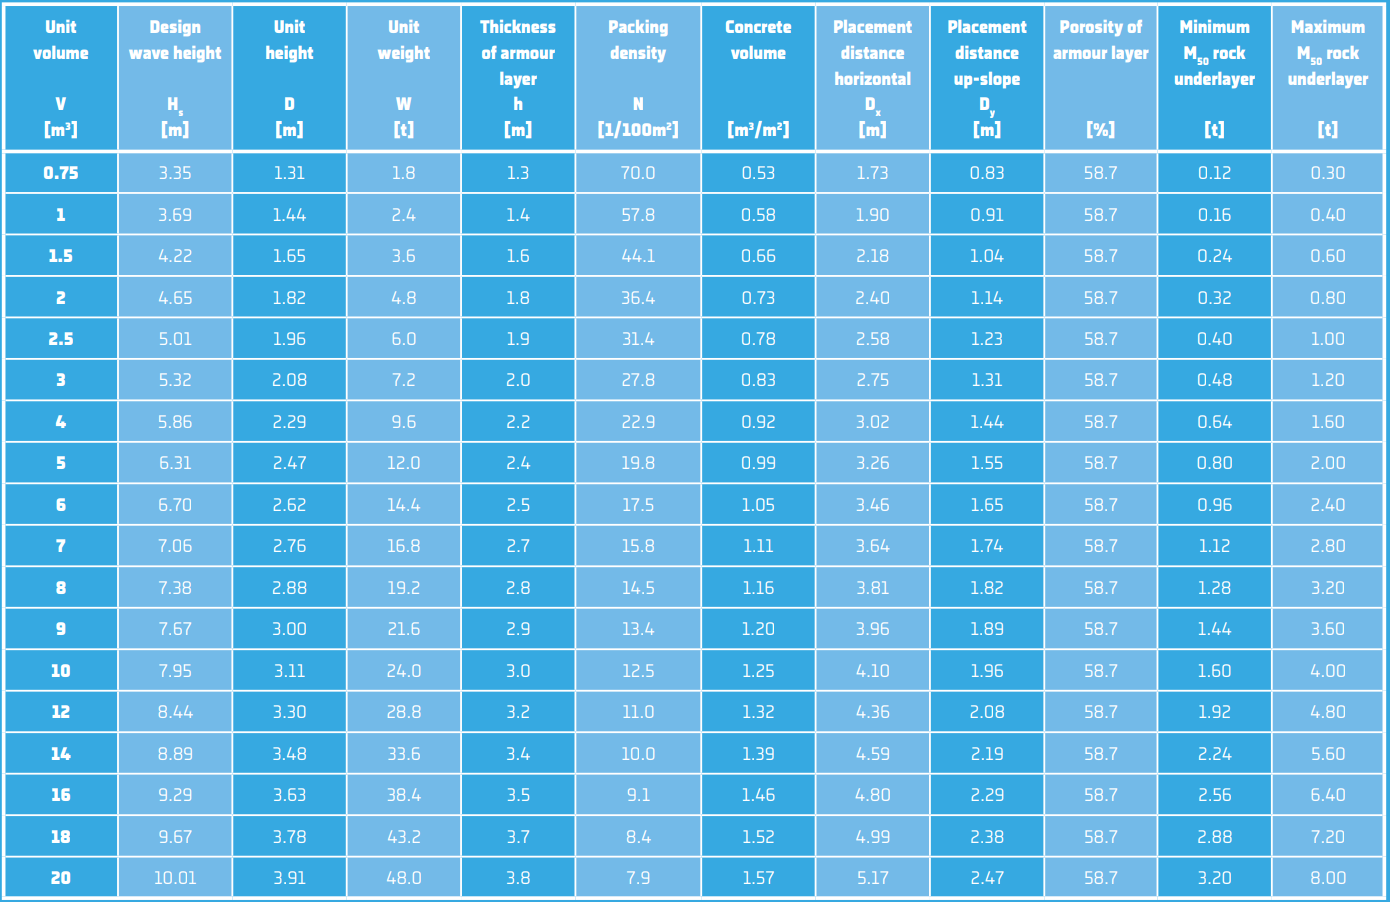
\includegraphics[width=\textwidth]{table53.png}
    \caption{Correction factors for local phenomena affecting 
    required X-Bloc unit size (DMC, 2023)}
    \label{fig:table53}
\end{figure}

The corrected volume was rounded up to the nearest standard unit 
size from Table 5-1 of the DMC guidelines to obtain the design 
volume $V_{design}$.

The maximum allowable number of rows on the slope is 20 for 
X-Bloc units, corresponding to a maximum slope length of 
$19\,D_y + 0.5\,D$, where $D_y$ is the upslope placement 
distance and $D$ is the unit height \cite{DMC2023}. If the 
slope length at the design water depth exceeds this limit, 
the unit size is increased until the constraint is satisfied. 
The slope length was computed as:

\begin{equation}
    L_{slope} = (h + \Delta_{HWL}) \times \frac{5}{3}
\end{equation}

for a 1:2 slope (cot$\alpha$ = 2) at the trunk and 1:3 slope 
(cot$\alpha$ = 3) at the head. The toe rock size was determined 
iteratively using the Van der Meer et al. (1995) formula 
\cite{DMC2023}:

\begin{equation}
    D_{n50} = \frac{H_s}{\left(2 + 6.2\left(\dfrac{h_t}{h}
    \right)^{2.7}\right) N_{od}^{0.15}\,\Delta}
\end{equation}

where $h_t = h - 3D_{n50}$ is the depth above the toe, and 
$N_{od} = 0.5$ corresponds to start of damage. The underlayer 
rock mass was checked to fall within the range of $W/6$ to 
$W/15$ of the unit mass as required by the DMC guidelines.

The rear face was designed symmetrically with the front armor 
as a conservative approach, since the relative freeboard 
$RFB = R_c/H_s > 1.5$ falls outside the standard guidance 
range of the DMC guidelines.
% -------------------- Results and Discussion --------------------
\section{Results and Discussion}
\subsection{Extreme Wave Statistics}
\hspace{0.5cm}

\subsection{Transformation of the Design Wave}
\hspace{0.5cm} 

\subsection{Design Water Level}
\hspace{0.5cm} 

\subsection{Run-up and Free Crest Height}
\hspace{0.5cm} 

\subsection{Armor Unit Selection and Design}
\subsubsection{Natural Rock}
\hspace{0.5cm}

\subsubsection{X-Bloc}
\hspace{0.5cm}

\subsection{Cross-Section Design}
\subsubsection{Section A-A}
\hspace{0.5cm}

\subsubsection{Section D-D}
\hspace{0.5cm}
% -------------------- Conclusion --------------------
\section{Conclusion}

\hspace{0.5cm}

\newpage

% -------------------- References --------------------

\begin{thebibliography}{99}
\addcontentsline{toc}{section}{References}

\bibitem{CE598}
Middle East Technical University, Department of Civil Engineering. (2025). \textit{CE 598 lecture notes} [Course notes].

\bibitem{CE593}
Middle East Technical University, Department of Civil Engineering. (2025). \textit{CE 593 lecture notes} [Course notes].

\bibitem{ERA5}
European Centre for Medium-Range Weather Forecasts. (n.d.). \textit{ERA5 reanalysis}. https://www.ecmwf.int/

\bibitem{shore}
U.S. Army Corps of Engineers. (1984). \textit{Shore protection manual}.

\bibitem{EurOtop2018}
Van der Meer, J.W., Allsop, N.W.H., Bruce, T., De Rouck, J., 
Kortenhaus, A., Pullen, T., Sch\"{u}ttrumpf, H., Troch, P., 
\& Zanuttigh, B. (2018). \textit{EurOtop: Manual on wave 
overtopping of sea defences and related structures} (2nd ed.). 
www.overtopping-manual.com.

\bibitem{DMC2023}
DMC. (2023). \textit{Xbloc \& XblocPlus design guidelines 2023}. 
Delta Marine Consultants.

\bibitem{}
Guler, H. G., Ergin, A., \& Ozyurt, G. (2014). A comparative 
study on the stability formulas of rubble mound breakwaters. 
\textit{Proceedings of the International Conference on Coastal 
Engineering 2014}.

\bibitem{}
Van der Meer, J. W. (1988). \textit{Rock slopes and gravel 
beaches under wave attack}. Delft Hydraulics.

\bibitem{}
Van der Meer, J. W. (2021). Updated rock stability formulae 
with spectral period. \textit{Journal of Coastal and Hydraulic 
Structures, 1}.

\bibitem{}
Van Gent, M. R. A., Van den Boogaard, H. F. P., Pozueta, B., 
\& Medina, J. R. (2007). Neural network modelling of wave 
overtopping at coastal structures. \textit{Coastal Engineering, 
54}(8), 586--593.



\end{thebibliography}
\newpage

% -------------------- Appendix --------------------
\appendix
\section{Appendix}

\subsection{Main MATLAB Code:}
\begin{lstlisting}[frame=single, numbers=left, style=Matlab-Pyglike]


\end{lstlisting}

\subsection{Distribution Constants Helper Function:}
\begin{lstlisting}[frame=single, numbers=left, style=Matlab-Pyglike]

\end{lstlisting}

\subsection{Fetch Calculation Python Code:}
\begin{lstlisting}[frame=single, numbers=left, language=Python, basicstyle=\ttfamily\scriptsize\small\color{black}]

\end{lstlisting}
\end{document}